\chapter{Einleitung}
\todo{Quellen Waschanlagen pro Jahr usw}
In Deutschland wird jedes Fahrzeug durchschnittlich 6 - 8 mal pro Jahr an einer der über 18.000 Waschanlagen gereinigt \cite{carwashpro}. Laut einer Studie der \ac{ica} nutzen Deutsche, verglichen mit fünf anderen europäischen Ländern, am häufigsten professionelle Waschanlagen \cite{ica}. 
Durch diese Gegebenheiten konnten Autowaschanlagen im Jahr 2021 deutschlandweit einen Umsatz von 1,43 Milliarden Euro erwirtschaften \cite{statista_umsatz}. 

\section{Otto Christ AG}
Mit circa 20.000 aktiven Anlagen in ganz Europa, sowie einem jährlichen Umsatz von 170 Millionen Euro, zählt die Otto Christ AG zu den führenden Herstellern in der Waschanlagenbranche \cite{christ}. Das familiengeführte Unternehmen beschäftigt aktuell circa 1600 Mitarbeitende und produziert jährlich bis zu 1000\footnote{Schätzung basierend auf den Verkäufen des Vorjahrs.} Waschanlagen. Von diesen werden über 60\% in andere Länder exportiert.
Um dabei den unterschiedlichen Kundenanforderungen gerecht zu werden, bietet die Firma verschiedene Maschinentypen an. Die automatische Wäsche von Personenkraftwagen wird durch \acp{pwa} oder Waschstraßen durchgeführt. Daneben besteht auch die Möglichkeit Nutzfahrzeuge mithilfe von Sonderwaschanlagen zu reinigen. In diese Kategorie fallen beispielsweise Lastkraftwagen, Busse und Züge. Eine steigende Kundenzahl bevorzugt nichtsdestotrotz die Wäsche von Hand gegenüber einer automatischen Maschine, weshalb auch \ac{sb}-Waschplätze angeboten werden.

Allen genannten Reinigungsvarianten ist gemeinsam, dass sie eine umfangreiche Menge Wasser verbrauchen. Wegen der zunehmenden Wichtigkeit des umwelttechnischen Aspekts, bietet die Otto Christ AG im Produktportfolio Wasseraufbereitungsanlagen an. Durch diese können bis zu 90\% des Brauchwassers wiederverwendet werden \cite{christ}. Ein weiteres ressourcenschonendes Angebot ist der Verkauf von generalüberholten Anlagen einer früheren Maschinengeneration. Bemerkenswert ist, dass die erste Waschanlage bereits im Jahr 1963 von \textit{Franz Christ} gebaut wurde \cite{christ}.

\newpage
\section{Aufbau einer Portalwaschanlage}
Die Grundidee der damaligen Waschanlage ähnelt dem Aufbau einer modernen \ac{pwa}, wie sie auf  \autoref{tikz:bertha} zu sehen ist. Bei diesem Maschinentyp steht das zu waschende Fahrzeug an einer festen Position, während sich die gesamte Anlage, im weiteren auch Portal genannt, über das Fahrzeug hinweg bewegt. Je nach Ausstattungsvariante der Waschanlage sind um das Portal herum verschiedene Düsen verbaut, mit denen Chemiezusätze zur Reinigung oder Frischwasser zum Klarspülen auf das Fahrzeug aufgebracht werden können. Durch oszillierende Hochdrucksysteme werden vor der Wäsche grobe Verunreinigungen entfernt. Anschließend kann die Oberfläche des Fahrzeugs durch die Seiten- und Dachbürste gründlich gereinigt werden. Die Räderwäscher hinter den Seitenbürsten werden zur Felgenreinigung eingesetzt. Nach der Wäsche wird das Fahrzeug durch seitliche Gebläse sowie einen bewegbaren Dachtrockner von überschüssiger Flüssigkeit befreit. 

Gesteuert wird die Waschanlage von einer \ac{sps} der Firma B\&R Industrial Automation GmbH. Zum Einsatz kommt hier typischerweise ein Modell der X-20 Serie, an das zusätzliche Schnittstellenmodule, wie digitale oder analoge Ein- und Ausgangskarten, angeschlossen werden können.
\begin{figure}[h!]
	\centering
	\begin{tikzpicture}[axis/.style={thin, black, ->, >=stealth', line width=0.2mm}, arrow style/.style={<-, thick}]
		\node[anchor=south west,inner sep=0] (image) at (0,0) {\includegraphics[width=0.88\textwidth]{pwa_seitlich2.jpg}};
		\begin{scope}[x={(image.south east)},y={(image.north west)}]
			\draw[arrow style] (0.37, 0.5) --(0.2,0.6) node[left] {Seitenbürste};
			\draw[arrow style] (0.45, 0.37) --(0.42, 0.19) node[below] {Fahrwerk};
			\draw[arrow style] (0.67, 0.91) --(0.75, 0.94) node[right] {Dachbürste};
			%\draw[help lines,xstep=.1,ystep=.1] (0,0) grid (1,1);
			%\foreach \x in {0,1,...,9} { \node [anchor=north] at (\x/10,0) {0.\x}; }
			%\foreach \y in {0,1,...,9} { \node [anchor=east] at (0,\y/10) {0.\y}; }
		\end{scope}
	\end{tikzpicture}
	\caption{CAD-Modell Portalwaschanlage C178}
	\label{tikz:bertha}
\end{figure}
\\
Im Rahmen dieser Arbeit werden die Bewegungen des Fahrwerks und der Seitenbürste näher betrachtet. 
Beide Baugruppen, im Weiteren auch als Module bezeichnet, sind auf \autoref{tikz:bertha} farbig hervorgehoben. 
Neben diesen sind noch drei weitere Baugruppen in der \ac{pwa} vorhanden, die über Hubeinrichtungen vertikal bewegbar sind. Davon ist nur die Dachbürste im Modell sichtbar, der Hochdruckbalken und die Dachdüse befinden sich vor bzw. hinter der grünen Seitenbürstenachse.
Die Kinetik der Module ist dabei vollständig von denen der anderen entkoppelt und erfolgt jeweils ausschließlich entlang der Achse, die ebenfalls farbig markiert ist. Bewegt werden die Module durch ihren zugehörigen Antriebsstrang, welcher im Folgenden beispielhaft beschrieben wird.

\subsection{Exemplarischer Aufbau eines Antriebsstrangs}
In diesem Unterabschnitt wird anhand des Fahrwerks beispielhaft der Aufbau eines Antriebsstrangs beschrieben. Die darin verbauten Komponenten sind der  \autoref{tikz:gantrydrive} zu entnehmen. Dieser Ausschnitt des CAD-Modells veranschaulicht die innere Struktur des Rot markierten Gehäuses auf der Gesamtübersicht (siehe  \autoref{tikz:bertha}). Angetrieben wird das System von einem Asynchronmotor. Dieser Motortyp ist in der Industrie am meisten verbreitet, da er in der Anschaffung günstig und dennoch sehr robust ist \cite{advanced_speed_control} \cite{electrical_drives}. Die Abtriebsdrehzahl des Motors wird durch ein nachgeschaltetes Getriebe mit Übersetzungsverhältnis $i>1$ reduziert, wohingegen das abgegebene Drehmoment um den selben Faktor erhöht wird\footnote{Bei idealisierter Annahme ohne Berücksichtigung des Wirkungsgrades}. Während bei allen Antriebssträngen Asynchronmotoren zum Einsatz kommen, unterscheiden sich die verwendeten Getriebetypen. Für das Fahrwerk wird ein Schneckengetriebe verwendet, das sich durch eine hohe Laufruhe auszeichnet \cite{tabellenbuch_metall}. Bei diesem sind die Ein- und Ausgangswelle um 90° versetzt angeordnet, sodass der Motor platzsparend verbaut werden kann (siehe  \autoref{tikz:gantrydrive}). Bei der Seitenbürste ist dagegen ein Zykloidgetriebe eingebaut, da hier wegen des begrenzten Bauraums Kompaktheit gefordert ist. Diese Getriebeart wird wegen ihrer Positioniergenauigkeit häufig in der Antriebstechnik eingesetzt \cite{zykliodgetriebe}.

Das vom Motor erzeugte und durch das Getriebe verstärkte Drehmoment bewirkt eine Winkelbeschleunigung der Laufrolle. Diese Beschleunigung resultiert in einer Veränderung der Drehzahl der Antriebsrolle, welche sich pro Umdrehung um ihren Umfang längs der Achse fortbewegt. 
Die zugrunde liegende Dynamik dieses Prozesses lässt sich modellhaft durch einen doppelten Integrator beschreiben. Die Variablen in  \autoref{tikz:antriebsstrang} sind nicht in Winkeleinheiten angegeben, da die Größen über den Umfang der Laufrolle auch auf den translatorischen Fall übertragbar sind. Außerdem wird statt dem erzeugten Drehmoment des Motors direkt die resultierende Beschleunigung angegeben, da diese zueinander proportional sind.
\begin{figure}[ht]
	\centering
	\begin{tikzpicture}[auto, node distance=2cm]
		\node (input) {};
		\node[IGlied, right of=input, node distance=3cm] (int1) {};
		\node[IGlied, right of=int1, node distance=3cm] (int2) {};
		\node[right of=int2, node distance=3.3cm] (output) {}; 
		\draw[->] (input) -- node[above] {$a$} (int1);
		\draw[->] (int1) -- node[above] {$v$} (int2);
		\draw[->] (int2) -- node[above] {$x$} (output);
	\end{tikzpicture}
	\caption{Wirkungsweise des Antriebsstrangs}
	\label{tikz:antriebsstrang}
\end{figure}
Die Bewegung der Antriebsrolle wird von einem Drehgeber gemessen, der auf der Abtriebsseite des Getriebes angebracht ist. Es handelt sich dabei um einen berührungslosen Sensor, der über den Hall-Effekt arbeitet. Dieser registriert die Winkeländerungen der Abtriebswelle, die über eine analoge Eingangskarte an der \ac{sps} erfasst werden. Es handelt sich also um ein inkrementelles Messsystem, weshalb jede Achse bei einem Neustart der \ac{pwa} zunächst über einen Endschalter referenziert werden muss.

Das auf \autoref{tikz:gantrydrive} dargestellte System ist, bis auf den Drehgeber, ebenfalls in gespiegelter Form auf der anderen Seite des Portals verbaut. Der zweite Sensor wird eingespart, da die Asynchronmotoren beider Seiten stets gleich angesteuert werden.
Die Kraftübertragung der Antriebsrolle auf das Grundgerüst des Portals erfolgt durch eine Rahmenkonstruktion, die auf  \autoref{tikz:gantrydrive} nicht dargestellt ist. Die Fahrschiene, entlang der diese Bewegung stattfindet, ist am Boden der Waschhalle befestigt und erstreckt sich über die gesamte Länge, typischerweise $7\, \text{m}$. Ebenfalls auf der Fahrschiene bewegt sich eine zweite Rolle, die sich am anderen Ende des Portalfußes befindet. Diese wird nicht angetrieben, sondern verhindert lediglich das Kippen des Portals. 
\begin{figure}[ht]
	\centering
	\begin{tikzpicture}[axis/.style={thin, black, ->, >=stealth', line width=0.2mm}, arrow style/.style={<-, thick}]
		\node[anchor=south west,inner sep=0] (image) at (0,0) {\includegraphics[width=0.63\textwidth]{antriebssystem.png}};
		\begin{scope}[x={(image.south east)},y={(image.north west)}]
			\draw[arrow style] (0.42, 0.38) --(0.23, 0.17) node[below] {\small Fahrschiene};
			\draw[arrow style] (0.12, 0.61) --(0.09, 0.48) node[below] {\small Lastrolle};
			\draw[arrow style] (0.57, 0.58) --(0.52, 0.66) node[above] {\small Laufrolle};
			\draw[arrow style] (0.81, 0.39) --(0.87, 0.31) node[below] {\small Getriebe};
			\draw[arrow style] (0.84, 0.49) --(0.89, 0.61) node[right] {\small Drehgeber};
			\draw[arrow style] (0.66, 0.82) --(0.61, 0.91) node[above left] {\small Asynchronmotor};
			%\draw[help lines,xstep=.1,ystep=.1] (0,0) grid (1,1);
			%\foreach \x in {0,1,...,9} { \node [anchor=north] at (\x/10,0) {0.\x}; }
			%\foreach \y in {0,1,...,9} { \node [anchor=east] at (0,\y/10) {0.\y}; }
		\end{scope}
	\end{tikzpicture}
	\caption{CAD-Modell Antriebsstrang Fahrwerk}
	\label{tikz:gantrydrive}
\end{figure}
Waschanlagen mit umfangreicher zusätzlicher Ausstattung weisen aufgrund ihres hohen Gewichts eine erhebliche Massenträgheit auf. Diese führt insbesondere während des Bremsvorgangs dazu, dass das Fahrwerk zum Rutschen neigt. Dabei kann es vorkommen, dass die Laufrolle übermäßig stark abgebremst wird und auf der Fahrschiene gleitet. Da der verbaute Drehgeber ausschließlich die Bewegung der Antriebsrolle erfasst, bleibt dieses Rutschen unbemerkt, da sich die Antriebsrolle wie vorgesehen verhält. Dadurch entsteht ein Positionsfehler, der erst erkannt wird, wenn die Achse erneut auf einen Endschalter trifft. In der Zwischenzeit könnte die unbemerkte Abweichung jedoch bereits zu Schäden an der Anlage oder des zu waschenden Fahrzeugs geführt haben. Die hohe Feuchtigkeit und chemischen Reinigungsmittel in der Waschhalle begünstigen dieses Verhalten. Um diesem Problem entgegenzuwirken, wird bei schweren Anlagentypen zusätzlich ein absolutes Messsystem in Form eines Seilzugsensors, verbaut. Auf diese Weise können die durch das Rutschen des Portals verursachten Abweichungen festgestellt werden.

\subsection{Ansteuerung des Frequenzumrichters}
Asynchronmotoren, die mit variabler Drehzahl betrieben werden sollen, erfordern aufgrund ihrer Bauweise den Einsatz eines Frequenzumrichters \cite{antriebstechnik}. Da deren Ansteuerung für das Verständnis der Arbeit notwendig ist, wird diese im Folgenden näher erläutert.

Je nach Antriebsstrang werden Motorsteuerungen eingesetzt, die sich in der Anschlussspannung und ihrer Nennleistung unterscheiden. Beispielsweise besitzt der Frequenzumrichter des Fahrwerks eine Nennleistung von $0,75\, \text{kW}$, wohingegen die Ansteuerung der  Seitenbürste $0,25\, \text{kW}$ aufweist \cite{schaltplan}. Zur Ansteuerung eines Asynchronmotors müssen dem Frequenzumrichter folgende motorspezifische Daten übergeben werden:
\begin{itemize}[before=\vspace{0.5em},after=\vspace{0.5em}]
	\item Nennspannung
	\item Nennfrequenz
	\item Nenndrehzahl
	\item Nennstrom
	%\item Cosinus $\varphi$
\end{itemize}
Für den Betrieb ist außerdem die Polpaarzahl des Motors relevant, diese berechnet der Frequenzumrichter aus der Nenndrehzahl, die bei Nennfrequenz erreicht wird. Diese Parameter werden in einer \ac{eds}-Datei gesichert und an die Motorsteuerung übertragen.

Die Kommunikation der \ac{sps} mit den Frequenzumrichtern findet dabei über das Bussystem CANopen statt. Durch dieses können zur Laufzeit definierte Parameter von der \ac{sps} oder dem Frequenzumrichter geschrieben, beziehungsweise gelesen, werden. Das funktionale Verhalten der Motorsteuerungen ist durch das CIA 402 Geräteprofil definiert \cite{lenze}. Darin wird eine Zustandsmaschine festgelegt, nach der der Frequenzumrichter arbeitet. Über die Variable \textit{controlword} kann die \ac{sps} in den gewünschten Zustand navigieren, dieser wird über das \textit{statusword} zurückgeben. Nur im Zustand \textit{Eingeschalten} ist eine Bewegung des Motors möglich.

Zur Definition der Motorbewegung stehen am Frequenzumrichter verschiedene Betriebsmodi zur Verfügung. Bisher wird der Motorsteuerung eine Geschwindigkeit, in Form einer Drehzahl, vorgegeben, die mit einer bestimmten Beschleunigung erreicht werden soll. 
Die Beschleunigung setzt sich dabei aus zwei Größen zusammen, und zwar der Geschwindigkeitsänderung $\Delta v$ und der Zeit $\Delta t$. Es ist zu beachten, dass für das Abbremsen des Motors andere Variablen als zur Beschleunigung gesetzt werden müssen. Die \textit{Acceleration} beschreibt, wie in \autoref{tikz:acceleration_fu} beispielhaft zu sehen, eine Erhöhung der Geschwindigkeit in positiver oder negativer Richtung. Dagegen wird mit \textit{Deceleration} eine Beschleunigung in Richtung der Ruhelage angegeben. 

\begin{figure}[ht]
	\centering
	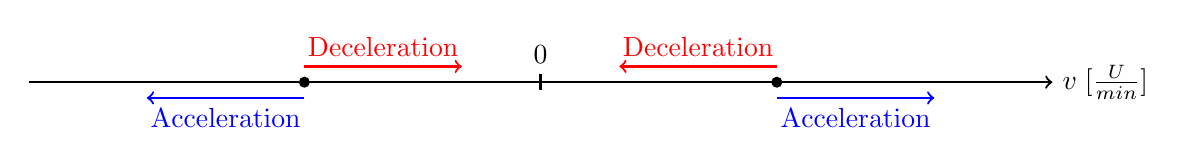
\begin{tikzpicture}
		\draw[thick,->] (-6.5,0) -- (6.5,0) node[anchor=west] {$v \; [\frac{U}{min}]$};
		\draw[thick] (0,-0.1) -- (0,0.1) node[anchor=south] {$0$};
		\fill (3,0) circle (2pt) node[anchor=north] {};
		\fill (-3,0) circle (2pt) node[anchor=north] {};
		
		\draw[->,thick,red] (3,0.2) -- (1,0.2) node[midway,above] {Deceleration};
		\draw[->,thick,red] (-3,0.2) -- (-1,0.2) node[midway,above] {Deceleration};
		\draw[->,thick,blue] (3,-0.2) -- (5,-0.2) node[midway,below] {Acceleration};
		\draw[->,thick,blue] (-3,-0.2) -- (-5,-0.2) node[midway,below] {Acceleration};
	\end{tikzpicture}
	\caption{Verwendung der Beschleunigungsvorgabe des Frequenzumrichters}
	\label{tikz:acceleration_fu}
\end{figure}

\newpage
\section{Relevanz der Verfahrgeschwindigkeit bei Waschanlagen}
\label{sec:motivation}
\todo{Hier könnte noch stehen dass bisher keine hohen Geschw möglich sind weil wir die aktuelle Position/Kontur des Autos nicht genau kennen}
Die Dauer eines Waschvorgangs ist aus wirtschaftlichen Gründen ein entscheidender Faktor für eine Waschanlage. Laut firmeninterner Quellen benötigt die Reinigung eines Autos aktuell durchschnittlich circa 12 Minuten. Die genaue Dauer ist abhängig vom gewählten Waschprogramm, sowie der Ausstattung des Portals. Dabei ist zu erwähnen, dass in Deutschland typischerweise kürzere Waschprogramme beliebter sind. Bei einer deutlichen Verkürzung der Wäsche, mit annähernd gleicher Qualität, würde ein Wettbewerbsvorteil gegenüber anderen Herstellern entstehen. 

\subsection{Grenzen der bisherigen Bewegungssteuerung}
Aufgrund limitierender Faktoren nutzen die Antriebe der \ac{pwa} aktuell in vielen Situationen nicht ihre theoretische Maximalgeschwindigkeit aus. Beispielsweise werden für viele Bewegungen die gleichen Lineargeschwindigkeiten verwendet, ohne die Länge der Strecke zu beachten. Dieses Verfahren ist nicht optimal, da auf längeren Strecken zwischenzeitlich eine höhere Geschwindigkeit gefahren werden könnte als auf kürzeren Strecken, sofern der Bremsweg eingehalten wird. Eine Optimierung dieser Verfahrgeschwindigkeit wurde bisher nicht realisiert, da dies eine exakte Regelung der Geschwindigkeit erfordert.

Die Messwerte des Drehgebers bzw. des Seilzugsensors würden zwar Informationen über die aktuelle Geschwindigkeit der Achse liefern, werden aber nicht für eine aktive steuerungsseitige Regelung dieser Größe verwendet. Stattdessen erfolgt die Vorgabe der gewünschten Geschwindigkeit direkt an die Motorsteuerung, welche unter Verwendung voreingestellter Beschleunigungswerte versucht, die Sollgeschwindigkeit zu erreichen. Die Berechnung der Stellgrößen für den Motor durch den Frequenzumrichter basiert auf einer U/f-Kennliniensteuerung (VFC open loop), wobei es sich um eine rein offene Steuerung ohne Rückkopplung handelt  \cite{lenze}.

Da der verwendete Antrieb ein Asynchronmotor ist, entsteht bauartbedingt ein unbekannter Schlupf während des Betriebs. Der Schlupf beschreibt die Drehzahldifferenz zwischen dem Stator- und dem Rotordrehfeld und somit die Abweichung der tatsächlichen Drehzahl von der vorgegebenen Soll-Drehzahl \cite{antriebstechnik}. Da diese Differenz nicht aktiv ausgeregelt wird, ist bislang keine präzise Geschwindigkeitskontrolle gewährleistet.\\
\\
Eine weitere Limitation stellt der derzeitige sequentielle Ablauf von Mehrachsenbewegungen dar. Dieser wird beispielsweise beim Trocknungsvorgang des Fahrzeugs deutlich, da hierbei immer nur eines der beteiligten Module in Bewegung ist: Das Fahrwerk wartet, bis der Dachtrockner die vorgegebene Höhe erreicht hat, ehe es zur nächsten Position losfährt. Anschließend hält der Dachtrockner an, bis das Fahrwerk die neue Position erreicht hat. Das schrittweise Vorgehen führt zu einem langsamen und unharmonischen Bewegungsablauf. Sollten die Bewegungen der Achsen jedoch präziser kontrollierbar sein, könnten optimierte Positionsverläufe, wie im nächsten Unterabschnitt beschrieben, Zeit einsparen.

\subsection{Optimierung des Positionsverlaufs}
Bisher gibt es zwei Möglichkeiten, die Fahrzeugkontur zu erfassen. Zum einen nutzen \acp{pwa} mit Standardausstattung den Anpressdruck der Waschbürsten, um das Fahrzeug schrittweise abzutasten. Für die Aufnahme der Seitenkontur fährt das Fahrwerk so lange auf das Fahrzeug zu, bis die Dachwalze den erforderlichen Anpressdruck erreicht hat. Anschließend fährt die Dachwalze eine definierte Strecke nach oben und das Fahrwerk wieder in Richtung Fahrzeug. Durch diesen Vorgang entstehen Punkte, mit denen die Kontur des Fahrzeugs beschrieben werden kann. Diese Punkte werden im Folgenden auch als Konturpunkte bezeichnet. Der Nachteil dieser Variante ist, dass nur sehr geringe Geschwindigkeiten verwendet werden können und die Fahrzeugkontur nur ungenau durch wenige Punkte beschrieben wird.

Um den Vorgang zu beschleunigen besitzen Waschanlagen mit gehobener Ausstattung der Firma Christ zusätzliche Messeinrichtungen, wie ein vertikal-angebrachtes Lichtgitter und seitliche Abstandsensoren. Damit wird die Höhen- und Seitenkontur des zu waschenden Fahrzeugs in einem ersten Überlauf \footnote{Ein Überlauf ist firmenintern als Bewegung des Portals über das Fahrzeug hinweg definiert.} erfasst, während bereits eine Vorwaschchemie aufgetragen wird. Die daraus gewonnen Konturdaten haben eine höhere Auflösung als die, die bei einer Abtastung des Fahrzeugs durch die Waschwalzen entstehende würden. Auf der Grundlage dieser Daten könnte auf der \ac{sps} nach dem ersten Überlauf ein glatteres Bewegungsprofil berechnet werden, was zu einem harmonischeren Ablauf der Wäsche führen würde. Bisher ist auch diese Optimierung nicht implementiert, da aufgrund der Geschwindigkeitsfehler ein korrektes Abfahren des Profils nicht gewährleistet werden kann. Stattdessen wird die feinere Auflösung der Daten genutzt, um mehr Konturpunkte in kleineren Schritten als beim Abtasten abzufahren. Wegen des Geschwindigkeitsfehlers wird auch während dieses Vorgangs der Anpressdruck der Waschbürsten ständig überprüft und gegebenenfalls wieder auf Abtastbetrieb umgeschaltet.

Ein weiterer Punkt zur Optimierung des Bewegungsablaufs wird am Beispiel des Starts eines Waschprogramms beschrieben.
Bei diesem bleibt das Fahrwerk in der Ruhestellung stehen, bis die Seitenbürsten in die Mitte und die Dachbürste nach unten gefahren sind. Erst nach Erreichen der Endpositionen beginnt das Fahrwerk mit der Bewegung in Richtung Fahrzeug. Dieser Prozess könnte dahingehend optimiert werden, dass das Fahrwerk bereits während der Bewegung der Bürsten verfährt und diese ihre Zielposition gleichzeitig erreichen. 

\subsection{Maximierung der Verfahrgeschwindigkeit}
Eine weitere Minimierung der Waschdauer, neben der Optimierung der Fahrwege, liegt in der Maximierung der Verfahrgeschwindigkeit. Bei einer präziseren Kontrolle der Achsgeschwindigkeiten könnte eine Berechnung durchgeführt werden, die den schnellstmöglichen Verlauf des optimierten Pfades als Lösung liefert. Dieser Verlauf könnte durch die Variablen Position, Geschwindigkeit und Beschleunigung definiert werden, da sich diese aus der Wirkungsweise des Antriebsstrangs (siehe \autoref{tikz:antriebsstrang}) ergeben und das System vollständig beschreiben.

Bei diesem Optimierungsproblem ist zu berücksichtigen, dass sich die vom Motor abgegebene Beschleunigung nicht unendlich schnell ändern kann. Damit die Achse der vorgegebenen Trajektorie folgen kann, muss daher die maximal zulässige Beschleunigungsänderung in der Planung beachtet werden. Außerdem sind die kinematischen Beschränkungen aller an der Bewegung beteiligten Achsen in der Berechnung zu berücksichtigen.

%Ein weiterer Vorteil der Trajektorienplanung besteht darin, die genaue Dauer der Bewegung bereits im Voraus zu berechnen. Der Endverbraucher sieht die verbleibende Zeit der Wäsche auf dem zugehörigen Eingabegerät der Waschanlage. Bisher beruhen die Werte jedoch ausschließlich auf Schätzungen und Erfahrungswerten.

\section{Aufgabenstellung}
\label{sec:aufgabenstellung}
Im Folgenden wird die Aufgabenstellung mit den dafür notwendigen Teilaufgaben konkretisiert. Ziel dieser Arbeit ist es, eine Regelung zu entwerfen, die eine verbesserte Kontrolle der Achsenbewegungen ermöglicht. Zu diesem Zweck sollen zwei Regelungskonzepte, ein Kaskadenregler und ein Zustandsregler, miteinander verglichen werden. Beide Regler müssen die Führungsgrößen Beschleunigung $a_{soll}$,  Geschwindigkeit $v_{soll}$ und Position $x_{soll}$ 
integrieren, da diese zukünftig von einer dynamischen Trajektorienplanung vorgegeben werden sollen, die auf einer vorherigen Pfadplanung basiert. Ziel des Reglers soll sein, dass die vorliegende Strecke diesen Vorgaben möglichst gut zu folgt. Als Messgröße steht die aktuell gemessene Position der Achse, ermittelt durch den Drehgeber, zur Verfügung. Der zusätzliche Seilzugssensor muss dabei nicht berücksichtigt werden, da nach dem Rutschen des Portals die Position des Drehgebers durch den absoluten Messwert auf der \ac{sps} automatisch angepasst wird.
Zur Verbesserung der Ansteuerung des Frequenzumrichter soll diese so verbessert werden, dass eine vorgegebene Beschleunigung als Eingangsgröße genutzt wird. Infolgedessen wird die Beschleunigung als Stellgröße des zu regelnden Systems fungieren.\\
\\
Da zum Start der Arbeit keine Pfad- und Trajektorienplanung vorhanden sind, sollen diese beispielhaft für eine festgelegte Bahn durchgeführt werden, um die Regelungskonzepte zu testen. Gemäß Aufgabenstellung des Unternehmens ist hierzu die Kontur der Zahl Acht zu verwenden. Der Grund für diesen speziellen Pfad ergibt sich aus einer Ähnlichkeit zur Autowäsche, welche in \autoref{sec:testbahn} genauer definiert wird. Für die Ausführung dieses Pfades ist die Bewegung zweier Achsen der \ac{pwa} erforderlich. Hierzu sollen das Fahrwerk und eine der Seitenbürsten eingesetzt werden. Sowohl der Start- als auch der Endpunkt der Bewegung liegen jeweils im Mittelpunkt der Acht. Auf Basis dieses Pfades soll anschließend eine Trajektorienplanung durchgeführt werden, die den schnellstmöglichen Bewegungsablauf berechnet. Dabei müssen maximale Geschwindigkeit- und Beschleunigungswerte der Achsen, sowie die Begrenzung der Beschleunigungsänderung eingehalten werden. Diese Stellgrößenbeschränkungen wurden durch firmeninterne Versuche ermittelt und werden als gegeben betrachtet (siehe \autoref{sec:bewegungsablauf}). Nach der Berechnung sollen die Ausgangsgrößen für beide Achsen zu jedem Zeitpunkt der Bewegung verfügbar sein. Diese dürfen nur Werte aufweisen, die von dem zugehörigen Antriebsstrang umgesetzt werden können.\\
\\
Zudem soll die modellhaft beschriebene Dynamik des vorliegenden Prozesses (siehe \autoref{tikz:antriebsstrang}) weiter untersucht werden, um ein Streckenmodell zu erstellen, welches den gesamten Antriebsstrang möglichst gut beschreibt. Anhand dieses Modells ist eine geeignete Simulationsumgebung zu erstellen, die es ermöglicht die Regelungskonzepte für diesen Anwendungsfall zu vergleichen. In der Simulation soll es möglich sein, typische Störgrößenverläufe zu untersuchen. Um die Versuchsergebnisse miteinander vergleichen zu können ist ein geeignetes Gütekriterium zu definieren.\\
\\
Im Anschluss soll das Regelungskonzept, welches in der Simulation die besten Ergebnisse liefert, auf dem realen Steuerungssystem implementiert werden. Die neue Regelung muss hierfür in die Bestandssoftware integriert werden. In diesem Schritt ist die Struktur des vorhandenen Programms zu analysieren, um herauszufinden an welcher Stelle es sinnvoll ist die Regelung einzuführen. Dabei müssen alle Anforderungen an die Softwareentwicklung der zugehörigen Abteilung eingehalten werden. Der Aufbau des Programms ist nach einem objektorientierten Ansatz zu gestalten. Es bietet sich an die Struktur anhand eines \ac{uml}-Diagramms zu visualisieren, ehe mit der Programmierung begonnen wird. Außerdem sollen für jede neue Klasse Unit-Tests erstellt werden, um die Funktionsfähigkeit der kleinsten testbaren Einheiten zu verifizieren und etwaige Fehler frühzeitig zu erkennen.\\
\\
Nach der Programmierung soll das Regelungskonzept an der physischen Anlage getestet werden. Eine Analyse der Testergebnisse, auch im Vergleich zur Simulation, ermöglicht die iterative Überarbeitung der Regelparameter. Die beiden Schritte sind mehrmals zu wiederholen, falls sich das Endergebnis dadurch weiterhin verbessert. Abschließend muss eine Validierung erfolgen, ob das ausgelegte Regelungskonzept für die klassischen Bewegungen einer \ac{pwa} geeignet ist, oder ob weitere Optimierungen des Reglers erforderlich sind.

\section{Stand der Technik}
\label{sec:stand_der_technik}
Um den aktuellen Stand der Technik zu beschreiben, wird im Folgenden erläutert, wie die Problemstellung der Arbeit typischerweise im industriellen Umfeld adressiert wird. Laut \cite{traj_s} wird das Thema Trajektorienplanung bereits seit Jahrzehnten untersucht und häufig in Kombination mit geschlossenen Regelkreisen eingesetzt. In dieser Quelle wird beschrieben, dass trapezförmige Geschwindigkeitsprofile eine effiziente Möglichkeit bieten, schnelle Bewegungen zu realisieren. Ein solches Profil ergibt sich, wenn die Soll-Geschwindigkeit durch eine konstante Beschleunigung erreicht wird, die Geschwindigkeit also linear ansteigt und ebenso durch eine konstante Beschleunigung wieder abgebremst wird.

Allerdings wird in \cite{traj_s} auch auf die damit verbundenen Nachteile hingewiesen. Dieses Bewegungsprofil führt durch sprunghafte Beschleunigungswechsel zu einem unendlich hohen Ruck. Dieser kann insbesondere bei mechanischen Komponenten die Lebensdauer verkürzen. Außerdem neigen diese Bewegungsprofile häufig zum Überschwingen.

Als alternative Lösung wird in der Literatur die Verwendung von s-förmigen Geschwindigkeitsprofilen vorgeschlagen \cite{traj_s}. Im Gegensatz zur trapezförmigen Geschwindigkeitsrampe wird die Geschwindigkeit hierbei durch ein Polynom dritten Grades modelliert. Die Ableitung dieser Funktion, also das resultierende Beschleunigungsprofil, weist keine Sprünge auf, sondern folgt einer Parabelform.\\
%Die Berechnung solcher Trajektorien ist unter anderem in \textit{MATLAB} mithilfe des \textit{Trapezoidal Velocity Profile Trajectory} Blocks implementierbar \cite{matlab_traj}.
\\
Ein alternativer Ansatz zur Regelung von Systemen ähnlicher Struktur wie in dieser Arbeit ist das Konzept der \textit{Flachheit}. Ein System wird als \textit{flach} bezeichnet, wenn sich sämtliche Zustandsvariablen sowie die Eingangsgrößen durch eine Funktion der Ausgangsgröße und einer endlichen Anzahl ihrer Ableitungen ausdrücken lassen \cite{flachheit}. Eine solche Ausgangsgröße wird als \textit{flacher Ausgang} bezeichnet.

Der entscheidende Vorteil dieses Ansatzes liegt darin, dass für eine gegebene Trajektorie des flachen Ausgangs die zugehörigen Trajektorien der Zustandsvariablen und Eingangsgrößen explizit berechnet werden können \cite{flachheit}. Dies ermöglicht eine direkte Bahnplanung und eine gezielte Steuerung des Systems durch die berechneten Führungsgrößen. Durch eine Zustandsrückführung kann auch eine Regelung des \textit{flachen} Systems realisiert werden. Zudem ist die flachheitsbasierte Regelung nicht auf lineare Systeme beschränkt, sondern kann auch auf nichtlineare Systeme angewendet werden, sofern die Zusammenhänge zwischen dem flachen Ausgang und den Systemzuständen mathematisch beschreibbar sind.
Generell eignet sich die Regelungsstruktur bei Anwendungen, die eine präzise Bewegungssteuerung erfordern.

\section{Struktur der Arbeit}
\todo{Kann das weg oder ist das Kunst?}
Die Ausarbeitung der Arbeit ist nach der Einleitung in vier Kapitel aufgeteilt. Zunächst wird auf Basis der Testbahn eine Pfad- und Trajektorienplanung durchgeführt, die als Ergebnis die optimierten Achsverläufe liefert. Anschließend wird das Streckenmodell näher untersucht, um es als Grundlage für die Simulation der Regelungskonzepte zu verwenden. Nach der Simulation wird das am besten geeignete Konzept in die bestehende Software integriert. Dazu wird zunächst die Struktur der Software analysiert. Abschließend wird das Regelungskonzept an der realen Anlage getestet und die erzielten Ergebnisse hinsichtlich ihrer Eignung für einen klassischen Waschablauf bewertet.
%\newlength{\colWidth}
%\setlength{\colWidth}{1.8mm}
%\newcommand{\weeks}[1]{\multicolumn{#1}{c}{\cellcolor{peuscherblau}}}
%\begin{flushleft}
%	\begin{table}[t]
%		\centering
%		\begin{tabular} {p{40mm} p{\colWidth}*{17}{p{\colWidth}}}
%			Kalenderwoche & 40 & 41 & 42 & 43 & 44 & 45 & 46 & 47 & 48 & 49 & 50 & 51 & 52 & 1 & 2 & 3 & 4 & 5 \\
%			\toprule[1.5pt]
%			Einarbeitung & \weeks{2}\\
%			\midrule
%			Trajektorienplanung & & & \weeks{1} \\
%			\midrule
%			Modellbildung   & & & \weeks{3}  \\
%			\midrule
%			Regelungssynthese & & & & & & \weeks{4}  \\
%			\midrule
%			Bewertung & & & & & & & & & \weeks{1}  \\
%			\midrule
%			Programmierung & & & & & & & & & & \weeks{5} \\
%			\midrule
%			Inbetriebnahme & & & & & & & & & & & & & & \weeks{3} \\
%			\midrule
%			Auswertung & & & & & & & & & & & & & & & &\weeks{2} \\
%			\midrule
%			Schriftl. Ausarbeitung & & & \weeks{16} \\
%		\end{tabular}
%		\caption{Zeitplanung Bachelorarbeit}
%		\label{tab:zeitplanung}
%	\end{table}
%\end{flushleft}









